\documentclass[12pt, titlepage]{article}

\usepackage{fullpage}
\usepackage[round]{natbib}
\usepackage{multirow}
\usepackage{booktabs}
\usepackage{tabularx}
\usepackage{graphicx}
\usepackage{float}
\usepackage{hyperref}
\usepackage{enumerate}
\usepackage{graphicx}
\hypersetup{
    colorlinks,
    citecolor=blue,
    filecolor=black,
    linkcolor=red,
    urlcolor=blue
}

%% Comments

\usepackage{color}

\newif\ifcomments\commentstrue %displays comments
%\newif\ifcomments\commentsfalse %so that comments do not display

\ifcomments
\newcommand{\authornote}[3]{\textcolor{#1}{[#3 ---#2]}}
\newcommand{\todo}[1]{\textcolor{red}{[TODO: #1]}}
\else
\newcommand{\authornote}[3]{}
\newcommand{\todo}[1]{}
\fi

\newcommand{\wss}[1]{\authornote{blue}{SS}{#1}} 
\newcommand{\plt}[1]{\authornote{magenta}{TPLT}{#1}} %For explanation of the template
\newcommand{\an}[1]{\authornote{cyan}{Author}{#1}}

%% Common Parts

\newcommand{\progname}{Software Engineering} % PUT YOUR PROGRAM NAME HERE
\newcommand{\authname}{Team 16, Durum Wheat Semolina
	\\ Alexander Moica
	\\ Yasmine Jolly
	\\ Jeffrey Wang
	\\ Jack Theriault
	\\ Catherine Chen
	\\ Justina Srebrnjak } % AUTHOR NAMES                 

\usepackage{hyperref}
    \hypersetup{colorlinks=true, linkcolor=blue, citecolor=blue, filecolor=blue,
                urlcolor=blue, unicode=false}
    \urlstyle{same}
                                


\newcounter{acnum}
\newcommand{\actheacnum}{AC\theacnum}
\newcommand{\acref}[1]{AC\ref{#1}}

\newcounter{ucnum}
\newcommand{\uctheucnum}{UC\theucnum}
\newcommand{\uref}[1]{UC\ref{#1}}

\newcounter{mnum}
\newcommand{\mthemnum}{M\themnum}
\newcommand{\mref}[1]{M\ref{#1}}

\begin{document}

\title{System Design for \progname{}} 
\author{\authname}
\date{\today}

\maketitle

\pagenumbering{roman}

\section{Revision History}

\begin{tabularx}{\textwidth}{p{3cm}p{2cm}X}
\toprule {\bf Date} & {\bf Version} & {\bf Notes}\\
\midrule
January 18, 2023 & 1.0 & Initial Document\\
April 02, 2023 & 1.0 & Revision 1 Changes\\
%Date 2 & 1.1 & Notes\\
\bottomrule
\end{tabularx}

\newpage

\section{Reference Material}

This section records information for easy reference.
\subsection{Relevant Documentation}
This document references multiple other documents that are listed below:

\begin{itemize}
	\item SRS, \cite{SRS}
	\item Development Plan, \cite{DevelopmentPlan}
	\item MG, \cite{MG}
	\item MIS, \cite{MIS}
\end{itemize}

\subsection{Abbreviations and Acronyms}

\renewcommand{\arraystretch}{1.2}
\begin{tabular}{l l} 
  \toprule		
  \textbf{symbol} & \textbf{description}\\
  \midrule 
  API & Application Programming Interface\\
  App & Application\\
  BMI & Body Mass Index\\
  CP & Cultural and Political Requirement\\
  FR & Functional Requirement\\
  LF & Look and Feel Requirement\\
  LR & Legal Requirement\\
  MG & Module Guide\\
  MIS & Module Interface Specification\\
  MS & Maintainability and Support Requirement\\
  OE & Operational and Environmental Requirement\\
  PR & Performance Requirement\\
  SR & Security Requirement\\
  SRS & Software Requirements Specification\\
  UH & Usability and Humanity Requirement\\
  \progname & Explanation of program name\\
  %\wss{...} & \wss{...}\\
  \bottomrule
\end{tabular}\\

\newpage

\tableofcontents

\listoftables

\listoffigures

\newpage

\pagenumbering{arabic}

\section{Introduction}


\subsection{Document Purpose}

This series of design documents are comprised of the System Design document, 
the Module Guide, and the Module Interface Specification. The purpose of these 
documents is to communicate the modular decomposition of 
the Utrition application, and provide readers with information regarding the 
functions/methods of each module, as well as the relationships between modules. 
Information about the high-level decomposition of modules can be found in 
the \href{../SoftArchitecture/MG.pdf}{MG}.
Details regarding each module's functions and methods are discussed in 
the \href{../SoftDetailedDes/MIS.pdf}{MIS}.

\subsection{System Purpose}

The purpose of Utrition is to provide users with an application that empowers 
them to discover the nutritional value of the foods they are consuming, and track
their previously eaten meals. Utrition takes a unique approach to the traditional nutritional logging applications by providing a variety of ways for users to input their food items into the application such as through text, verbal communication, and image. Users with keyboard-typing accessibility concerns will have a nutritional logging application that they can use without external assistance.

\subsection{Scope}

Users will be able to input their food items to Utrition by using speech to text, typing, or uploading food images to the front-end user interface. If users would like to upload an image of the food they want nutritional information for, they would have to provide a photo of the food on the device using Utrition. This can be done by downloading an image of the food item onto the user's device (i.e. computer). After user input, Utrition will begin internal calculations to obtain nutritional information for the food item from the public Nutritionix API. The nutritional information will be provided to the front-end user interface for the user to view.

\wss{Include a figure that show the System Context (showing the boundary between
your system and the environment around it.)}

\begin{figure}[H]
	\centering
	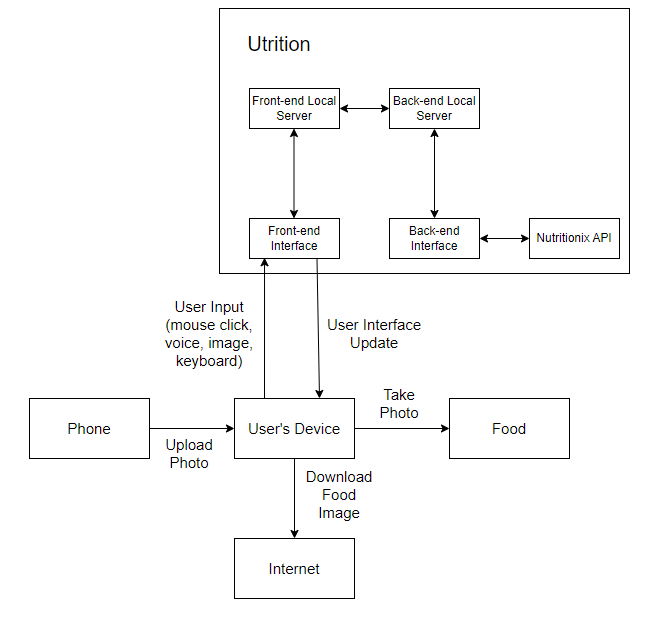
\includegraphics[scale=0.8]{System_Context_Diagram.png}
	\caption{System Context Diagram}
\end{figure}


\section{Project Overview}

\subsection{Normal Behaviour}

In their command-line interface, users will travel to the Utrition directory. From there, users will enter commands ``npm start" and ``npm run start-backend" separately. Utrition's front-end and back-end interfaces will successfully connect to the user's localhost server. Users will be greeted with Utrition's home page. They may travel to their profile page, where they can find their past nutritional data saved in a list. On this page, users may decide to view their nutritional trends in graph form. Users may also travel to the upload page, where they can input food item(s) to find their nutritional information. Users can input food items by 
\begin{itemize}
	\item Clicking on the search bar and typing in the food items. Each food item is separated by a comma.
	\item Clicking on the microphone button and verbally listing the food items.
	\item Clicking on the upload button and then selecting an image of a food item.
\end{itemize}
Users finalize their search by clicking the search button. In return, the user will be shown the nutritional information for each food item searched. The nutritional information is acquired by utilizing the Nutritionix public API. The data is stored on the user's device, so that past nutritional trends can be viewed on their profile page.

\subsection{Undesired Event Handling}

\wss{How you will approach undesired events}

A more in-depth look to Utrition's undesired event handling can be found in Utrition's \href{../../HazardAnalysis/HazardAnalysis.pdf}{Hazard Analysis} document.

In all cases except for one, the Utrition front-end interface will notify the user of the issue disrupting normal use of the application. Most of these errors will be detected by the back-end interface of Utrition. As a result, the application's back-end interface will send the error message to the front-end interface through the user's local server for the front-end interface to display. Certain errors, such as incorrect image type, are detected by the front-end interface and will not have to travel through the local servers to deliver the error message to the user. 

The one specific case where Utrition will not notify the user of the specific error is when Utrition closes unexpectedly. The cause of this rare issue is unknown to the developers, but the application will save its data periodically during use to ensure minimal information is lost from the crash.

\subsection{Component Diagram}
\newpage
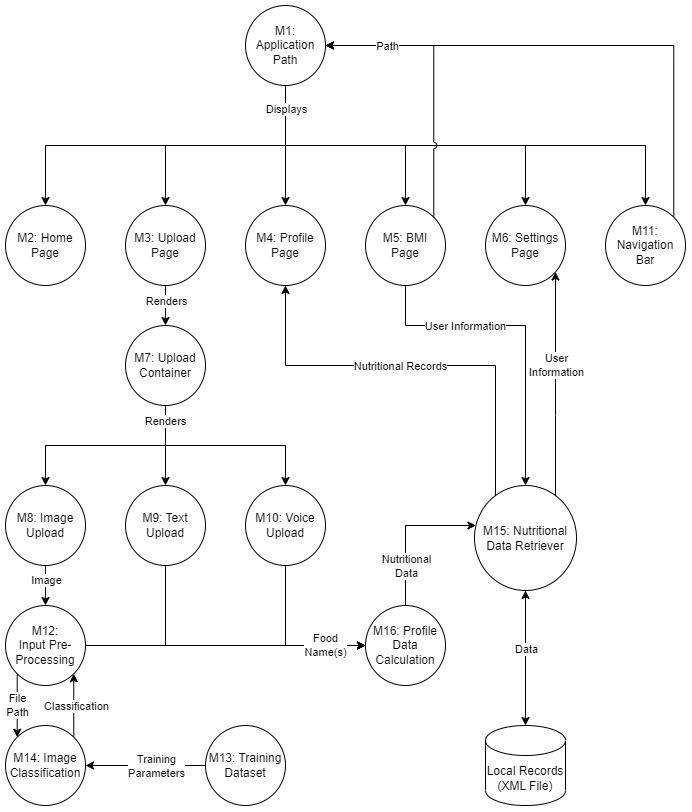
\includegraphics[scale=0.63]{componentdiagram.jpg}

\subsection{Connection Between Requirements and Design} 

\wss{The intention of this section is to document decisions that are made
  ``between'' the requirements and the design.  To satisfy some requirements,
  design decisions need to be made.  Rather than make these decisions implicit,
  they are explicitly recorded here.  For instance, if a program has security
  requirements, a specific design decision may be made to satisfy those
  requirements with a password.}

\subsubsection{Functional Requirements}

\begin{enumerate}[{FR}1. ]
	\item Provide the user with an interface that has the option to select the type of input as image upload. The user can then select an image file from their computer that they can submit as input.
	\item The food item(s) uploaded to the Utrition front-end will be condensed to a 32x32 pixel image, which is then turned into a 32x32 array. The array containing data for each pixel is then transferred to the Utrition back-end. From there, the image is parsed through a TensorFlow machine learning algorithm which is trained on the CIFAR-100 dataset to determine the food item.
	\item The Utrition back-end provides the Nutritionix API with valid headers (x-app-id, x-app-key, x-remote-user-id) that allow the use of the API (retrieval of nutrition facts).
	\item The Utrition back-end interface sends a POST request to the Nutritionix API. The response to the POST request provides the back-end interface with a JSON file containing the food’s macro-nutrients, micro-nutrients, and caloric details.
	\item Once the Utrition back-end has received the nutritional details of the food item from the Nutritionix API, the back-end stores the nutritional information in a CSV file in the users’ Utrition folder.
	\item Once the user requests to see past nutritional data, the front-end interface sends a GET request to the front-end local server. This request is passed to the back-end local server, which then gets sent to the back-end interface. The back-end interface returns the data of all logged entries in the previously logged food items CSV file to the front-end interface (going through their respective local servers). The front-end interface displays the file's data in reverse-chronological order.
	\item Once the Utrition back-end interface receives the JSON file from the Nutritionix API, the data is sent to the local back-end server, to the local front-end server, and then to the front-end interface. In the front-end interface, the JSON file has the “stringify” method applied to it to display the information to the user.
	\item Provide the user with an interface that has the option to select the type of input as text upload. The user can then type in their food items that they can submit as input.
	\item The text input field will be able to accommodate large amounts of text to be submitted where more than one food item can be specified.
	\item Provide the user with an interface that has the option to select the type of input as voice upload. The user can then vocalize their food items that they can submit as input.
	\item The voice input field will be able to accommodate large amounts of audio to be submitted where more than one food item can be specified.
	\item The audio input that the user submits will be translated to text using ``react-hook-speech-to-text" package.
	\item A ``reset" button will be created on the voice input interface to allow the user to clear their previous audio input.
	\item The Utrition back-end interface sends a POST request to the Nutritionix API containing all the text inputted by the user (from text input or voice input). The Nutritionix API is able to parse the text for food items. The response to the POST request provides the back-end interface with a JSON file containing each identified food and the corresponding macro-nutrients, micro-nutrients, and caloric details.
	\item The front-end interface will contain buttons for the user to switch between each upload option.
	\item Once the user requests to see past nutritional data found on the ``Profile" page, the front-end interface sends a GET request to the front-end local server. This request is passed to the back-end local server, which then gets sent to the back-end interface. The back-end interface returns a JSON-formatted string that contains the user's most eaten food item to the front-end interface (going through their respective local servers). This food item is found by finding the mode of all the food entries saved in the past food entries CSV file.
	\item Once the user requests to see past nutritional data found on the ``Profile" page, the front-end interface sends a GET request to the front-end local server. This request is passed to the back-end local server, which then gets sent to the back-end interface. The back-end interface returns a JSON-formatted string that contains the total calories inputted for the current day to the front-end interface (going through their respective local servers). This caloric value is found by adding all the calories within food entries in the past food entries CSV file that have the current date.
	\item Once the user requests to see past nutritional data found on the ``Profile" page, the front-end interface sends a GET request to the front-end local server. This request is passed to the back-end local server, which then gets sent to the back-end interface. The back-end interface returns a JSON-formatted string that contains a list of JSON formatted strings with the date, total calories per day, and all the foods eaten on that day to the front-end interface (going through their respective local servers). This list is constructed by iterating over all the food entries in the past food entries CSV file. During this iteration, a list will be constructed to keep track of all foods consumed on one day and a float sum will add all calories for one day.
	\item The back-end interface will be able to access the CSV file directly. This will allow calculations for the total calories per day and creating list subsets for the foods consumed on a certain day.
	\item A navigation bar is provided at the top of every page.
	\item Once the user is located on the ``Profile" page, a ``delete" button will be available for each past food entry input. When a user confirms they want to delete a specified entry, the front-end interface sends a POST request to the front-end local server. This request is passed to the back-end local server, which then gets sent to the back-end interface. The back-end interface will delete the identified food entry from the past food entries CSV file.
	\item A front-end interface will be provided to the user where they can input their personal statistics. This includes their age, weight, height, gender, and activity level.
	\item Once the user inputs their personal statistics and presses a ``submit" button, a POST request is sent to the front-end local server. This request is passed to the back-end local server, which then gets sent to the back-end interface. The back-end interface will save all user statistics in a JSON file that can be accessed for future calculations.
	\item The user will be able to resubmit their user statistics after they have initially been saved. This is done by filling out the input fields with different values and clicking the ``submit" button. The remaining process follows the FR23 design decision.
	\item Once the JSON file with user statistics is available, the backend-interface will be able to access these values directly. Simple calculations can be done to find the user's BMI and recommended calories.
	\item Once the user is located on the ``Profile" page, the BMI related calculations will be displayed. This is done when the front-end interface sends a GET request to the front-end local server. This request is passed to the back-end local server, which then gets sent to the back-end interface. The back-end interface will return a JSON-formatted string that contains the user's BMI and recommended calories.
	\item Once the user is located on the ``Profile" page, the front-end interface sends a GET request to the front-end local server. This request is passed to the back-end local server, which then gets sent to the back-end interface. The back-end interface creates a graph of the date versus the total calories for that each date. This is done using the python package ``plotly". The graph is saved as .png image that the front-end interface can access directly.
	\item Once the user is located on the ``Profile" page and clicks the ``delete" button for a past food entry, a confirmation button will be displayed to the user. The specified entry will only be deleted once the user has given confirmation since deletion is an irreversible action. 
\end{enumerate}

\subsubsection{Non-Functional Requirements}
\begin{enumerate}[{LF}1. ]
	\item Front end developers will make a conscious effort not to place different components near each other. If components are determined to be close in proximity by the developers, \href{https://www.rapidtables.com/web/tools/pixel-ruler.html}{a pixel measuring tool} will be used to determine the distance between components.
\end{enumerate}

\begin{enumerate}[{UH}1. ]
	\item A navigation bar is provided at the top of every page.
	\item This design decision is covered by FR5's design decision.
	\item Utrition will provide steps on how to use the product on its home page. Utrition will not provide the user with many available actions, so it becomes clear to individuals how to use the product. 
	\item Nutritional information (calories, fat, sodium, carbohydrates, sugar, and protein) will have appropriate units.
	\item Only important nutritional information is displayed to the user (calories, fat, sodium, carbohydrates, sugar, and protein) and back-end calculations are not displayed to the user. Front end reformatting of information will not be displayed to the user as well.
	\item No sound files will be found in Utrition's GitHub repository.
\end{enumerate}

\begin{enumerate}[{PR}1. ]
	\item Each screen loads in their personal set of functions. Each screen will not load in many functions.
	\item The machine learning algorithm sets the maximum amount of iterations to be 1000 for each image.
	\item The Nutritionix API will provide correct results to the back-end system, which then gets sent to the front-end interface through their respective local servers unless the user does not have an internet connection or an obscure food item is entered.
	\item Utrition is a local web application that can be run by an infinite amount of people at the same time. There is no server to restrict user access.
	\item Once Utrition is fully developed with no code errors, any person will be able to access and run Utrition. The application will be indefinitely available on GitHub.
\end{enumerate}

\begin{enumerate}[{OE}1. ]
	\item Utrition is available on GitHub.
	\item The user guide will be indefinitely available on GitHub. The document will be written in simple English phrases for all people aged 14 and older to understand.
	\item No developers will make changes to Utrition after publication.
\end{enumerate}

\begin{enumerate}[{MS}1. ]
	\item The CIFAR-100 dataset can be swapped with another appropriate dataset by placing it under the src/utrition-backend/ML/ folder.
	\item Developers will upload a user guide which includes installation and usage instructions on the Utrition GitHub.
	\item The application will be available on all Windows, macOS, and Linus devices.
\end{enumerate}

\begin{enumerate}[{SR}1. ]
	\item Utrition and all source code files are available as a public repository on GitHub.
	\item After every food input, Utrition will save the item(s) and corresponding nutritional data in a CSV file.
	\item Utrition only stores previously searched food items’ nutritional information on the users’ Utrition folder. Utrition does not communicate with other instances of Utrition on other devices.
\end{enumerate}

\begin{enumerate}[{CP}1. ]
	\item Developers will not include any potentially insensitive content.
\end{enumerate}	

\begin{enumerate}[{LR}1. ]
	\item Developers will not include any malicious software in Utrition.
	\item Development of Utrition will be done on GitHub.
	\item GitHub’s CI/CD pipeline will be used with Pylint. Developers will review the results of the Pylint test to determine if coding conventions are not being followed properly.
	\item Front-end developers code in ReactJS and CSS using Google’s style guide. A review is performed by the front-end developers before the final launch of Utrition.
	\item Front-end developers design the interface using Google’s style guide. A review is performed by the front-end developers before the final launch of Utrition.
\end{enumerate}	
\section{System Variables}

\wss{Include this section for Mechatronics projects}

\subsection{Monitored Variables}

N/A

\subsection{Controlled Variables}

N/A

\subsection{Constants Variables}

N/A

\section{User Interfaces}

\wss{Design of user interface for software and hardware.  Attach an appendix if
needed. Drawings, Sketches, Figma}


\includegraphics[scale=0.55]{home.jpg}\\ \\
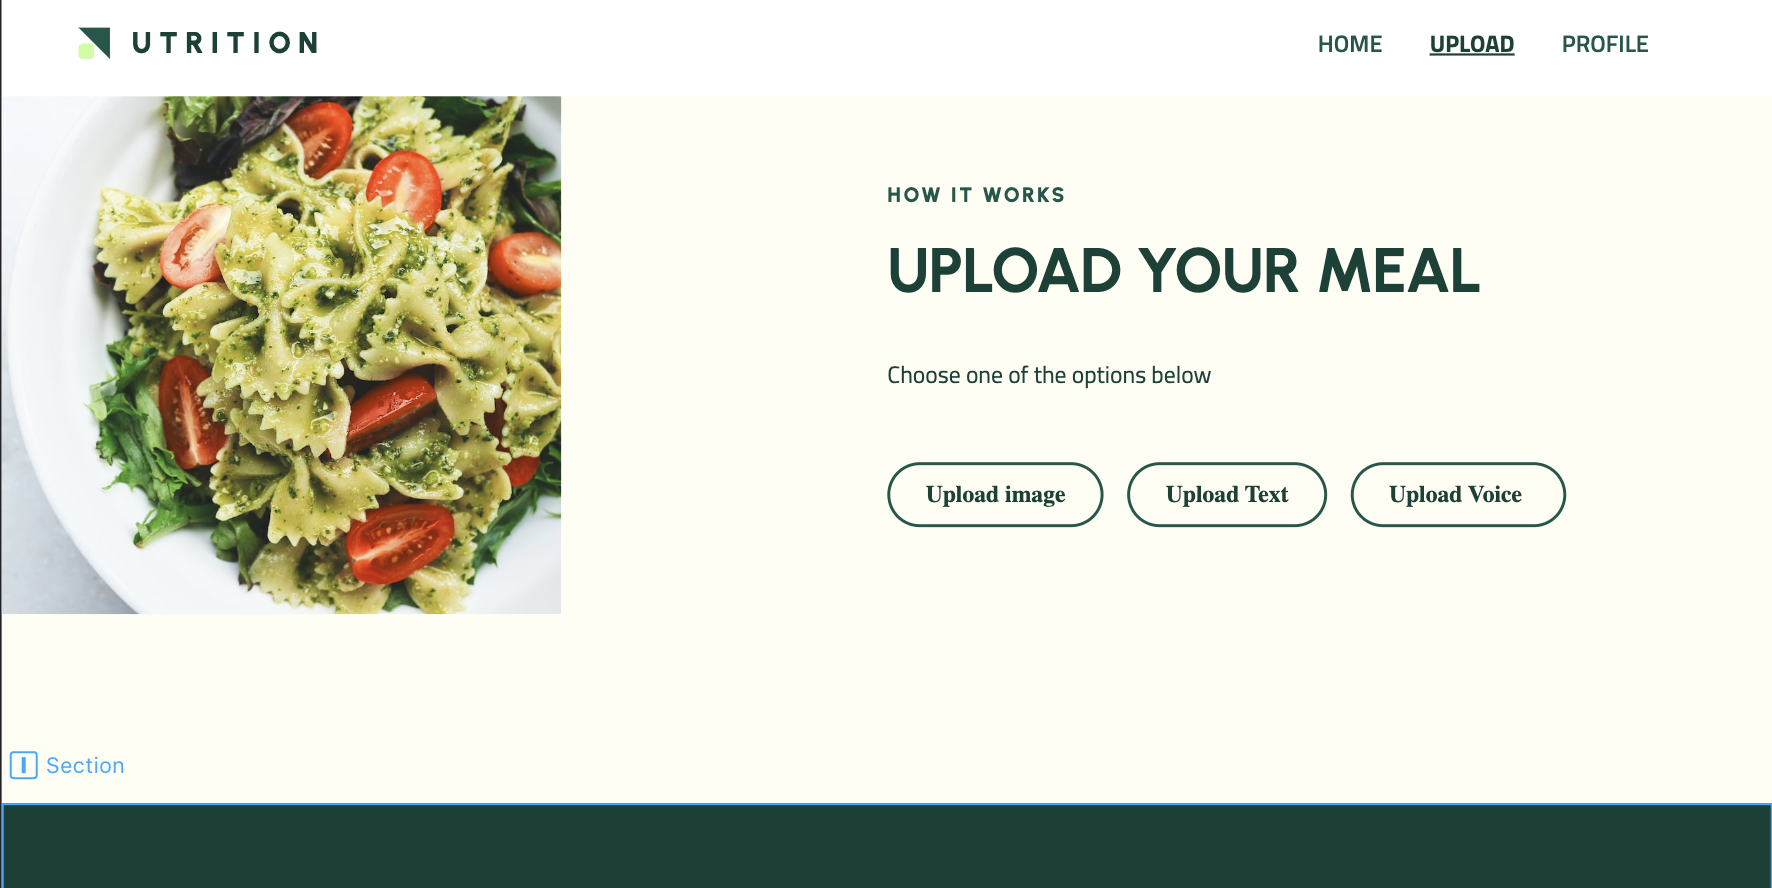
\includegraphics[scale=0.55]{upload.jpg}\\
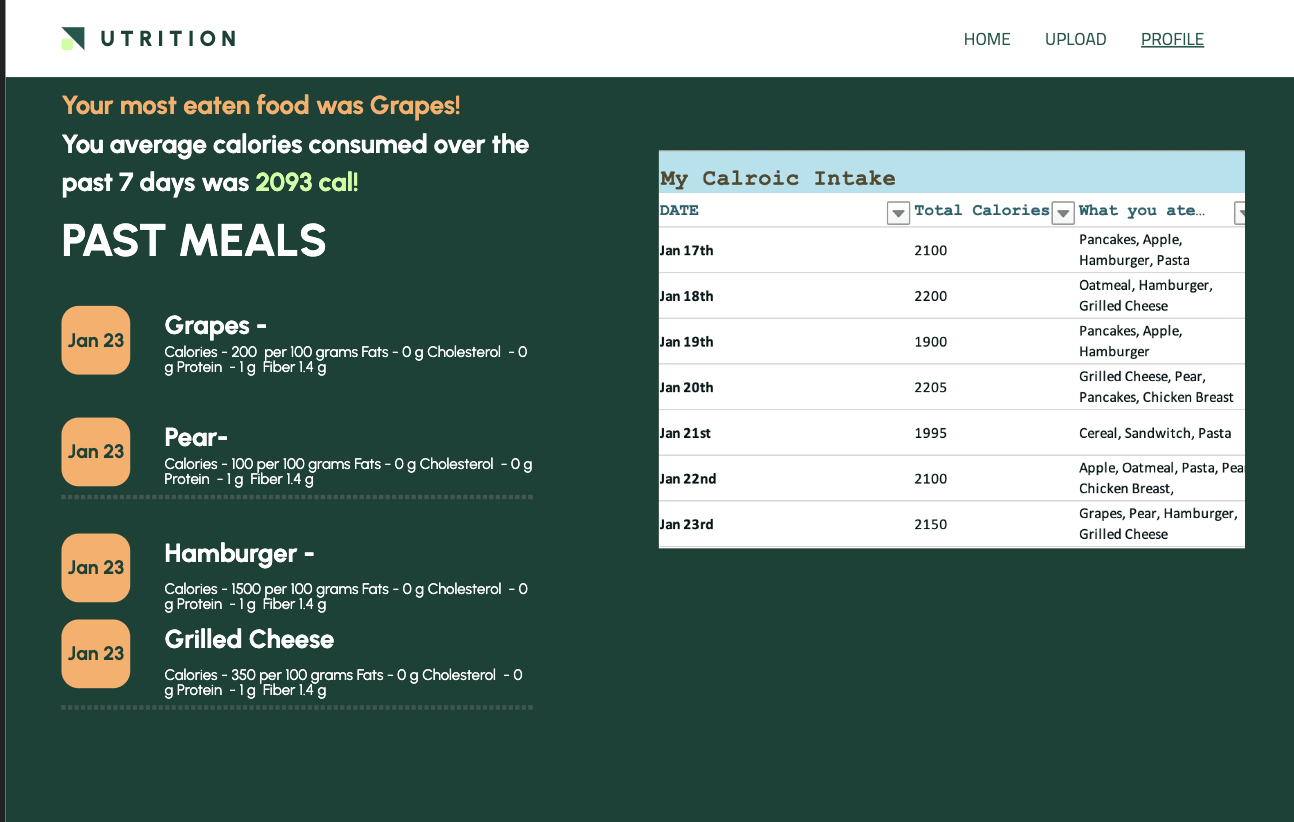
\includegraphics[scale=0.75]{profile.jpg}

\section{Design of Hardware}

\wss{Most relevant for mechatronics projects}
\wss{Show what will be acquired}
\wss{Show what will be built, with detail on fabrication and materials}
\wss{Include appendices as appropriate, possibly with sketches, drawings, CAD, 
etc}

N/A

\section{Design of Electrical Components}

\wss{Most relevant for mechatronics projects}
\wss{Show what will be acquired}
\wss{Show what will be built, with detail on fabrication and materials}
\wss{Include appendices as appropriate, possibly with sketches, drawings,
circuit diagrams, etc}

N/A

\section{Design of Communication Protocols}

\wss{If appropriate}

To use Utrition, users must run commands “npm start” and “npm run start-backend”. The “npm start” command allows for the front-end user interface to be displayed and connects the front-end interface to the user’s local server (http://localhost:3000). The “npm run start-backend” command creates an unseen back-end interface on the user’s local server (http://localhost:5000). Since the front-end and back-end connect to the same local server with different ports, communication is done by the front-end sending GET and POST requests to the front-end local server, which is then read by the connecting back-end local server. The back-end interface receives the GET or POST request from the back-end local server and begins working on the given task. Once the task has been completed, the back-end returns data through the local server to reach the front-end (which is waiting for the back-end’s response). For example, if the request from the front-end is to find nutritional data for a food item, the front-end will send a GET request to the local server. The back-end reads this GET request from their local server (because they are located at the same address) and sends a POST request to the Nutritionix API. In return, the Nutritionix API will deliver the data back to the back-end. From there, the back-end returns the Nutritional data to the front-end by using the local server. 


\section{Timeline}

\wss{Schedule of tasks and who is responsible}

\begin{table}[H] 
	\begin{tabularx}{\textwidth}{|X|X|X|}
		\hline
		\textbf{Module} & \textbf{Main Developer} & \textbf{Due Date}\\
		\hline
		Training Dataset & Alex Moica & 
		Completed \\
		\hline
		Input Pre-Processing & Alex Moica & 
		Completed \\
		\hline
		Image Classification & Alex Moica & 
		Completed \\
		\hline
		Nutritional Data Retriever & Catherine Chen & 
		Completed \\
		\hline
		Voice Upload  & Catherine Chen & 
		Completed \\
		\hline
		Application Path & Jeffrey Wang & 
		Completed \\
		\hline
		Navigation Bar & Jeffrey Wang & 
		Completed \\
		\hline
		Image Upload  & Jeffrey Wang & 
		Completed \\
		\hline
		Back-end Communication & Justina Srebrnjak & 
		Completed \\
		\hline
		Food Entry & Justina Srebrnjak & 
		January 25th, 2023 \\
		\hline
		Upload Page & Yasmine Jolly & 
		January 25th, 2023 \\
		\hline
		Profile Page & Jack Theriault & 
		January 28th, 2023 \\
		\hline
		Manual Logging  & Yasmine Jolly & 
		January 29th, 2023 \\
		\hline
		User Log Data Structure & Justina Srebrnjak & 
		February 1st, 2023 \\
		\hline
		Nutrition Log & Jack Theriault & 
		February 4th, 2023 \\
		\hline
		Home Page & Yasmine Jolly & 
		February 4th, 2023 \\
		\hline
		Extensive Manual Testing Of Each Module & Catherine Chen & 
		February 5th, 2023 \\
		\hline
	\end{tabularx}
	\caption{Module Timeline}
\end{table}

\bibliographystyle {plainnat}
\bibliography{../../../refs/References}

\newpage{}

\appendix

\section{Interface}

\wss{Include additional information related to the appearance of, and
interaction with, the user interface}

\section{Mechanical Hardware}

N/A

\section{Electrical Components}

N/A

\section{Communication Protocols}

\begin{figure}[H]
	\centering
	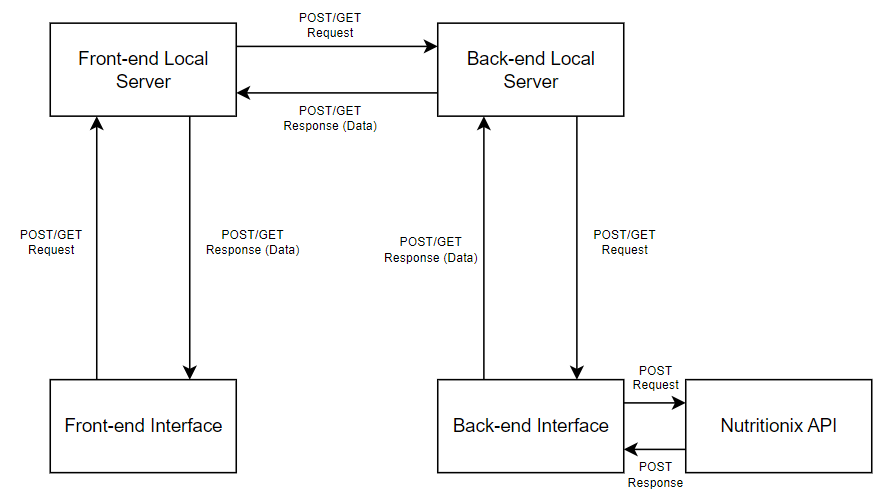
\includegraphics[scale=0.85]{Communication_Protocols.png}
	\caption{Communication between the front-end and back-end}
\end{figure}

\section{Reflection}

The information in this section will be used to evaluate the team members on the
graduate attribute of Problem Analysis and Design.  Please answer the following questions:

\begin{enumerate}
  \item What are the limitations of your solution?  Put another way, given
  unlimited resources, what could you do to make the project better? (LO\_ProbSolutions)
  \item Give a brief overview of other design solutions you considered.  What
  are the benefits and tradeoffs of those other designs compared with the chosen
  design?  From all the potential options, why did you select documented design?
  (LO\_Explores)
\end{enumerate}

The Utrition development team has identified some shortcomings of our project. Firstly, Utrition utilizes the CIFAR-100 dataset to identify food items with TensorFlow, a machine learning algorithm. However, the CIFAR-100 dataset only contains 5 identifiable food items. With unlimited resources, the Utrition team would find a larger dataset containing a bigger variety of food items. With this larger dataset, our application would be able to identify many more food items with higher confidence. In addition to the improved machine learning technology, the application's aesthetic display could be improved to be more visually appealing and intuitive. Most notably, the front-end developers would add charts and diagrams to display a user's previous meals rather than listing them.

The original design for Utrition was to identify a food item from one form on input. This method required uploading an image that would utilize machine learning for identification. This input method was chosen since uploading an image is simple and doable for all age groups. However, the trade-off was that complex food items, such as full meals (not only simple ingredients), would be impossible for the algorithm to identify given our training dataset. As a result, users would quickly get frustrated with the near-useless application. Therefore, the developers behind Utrition decided that it was best to provide more searching options (textual and verbal input) to the user even if it came with the price of adding more clutter to the user interface. The developers did not simply want to add an option to type the food item, as those with accessibility concerns may struggle to type the food item correctly. Therefore, the developers decided it was best to provide the user with all three input options, so the users could decide what method was best for them and their goals.

\end{document}